\section{Aufgabe 2}
In dieser Aufgabe Soll der Frequenzgang an 3 Lastwiderständen gemessen werden. Diese könnten z.B. Lautsprecher repräsentieren, die jeweils Wechselstrom mit verschiedenen Frequenzen in Schallwellen umwandeln können. Gemessen wird also die Effektivspannung am Funktionsgenerator \(U_G\) und die jeweiligen Effektivspannungen an den Lastwiderständen \(U_i\). 
\subsection{Aufbau}
Um sich den Aufbau besser vorstellen zu können hier das Schaltbild:
\begin{center}
\begin{minipage}{\linewidth}
\centering
\makebox[0cm]{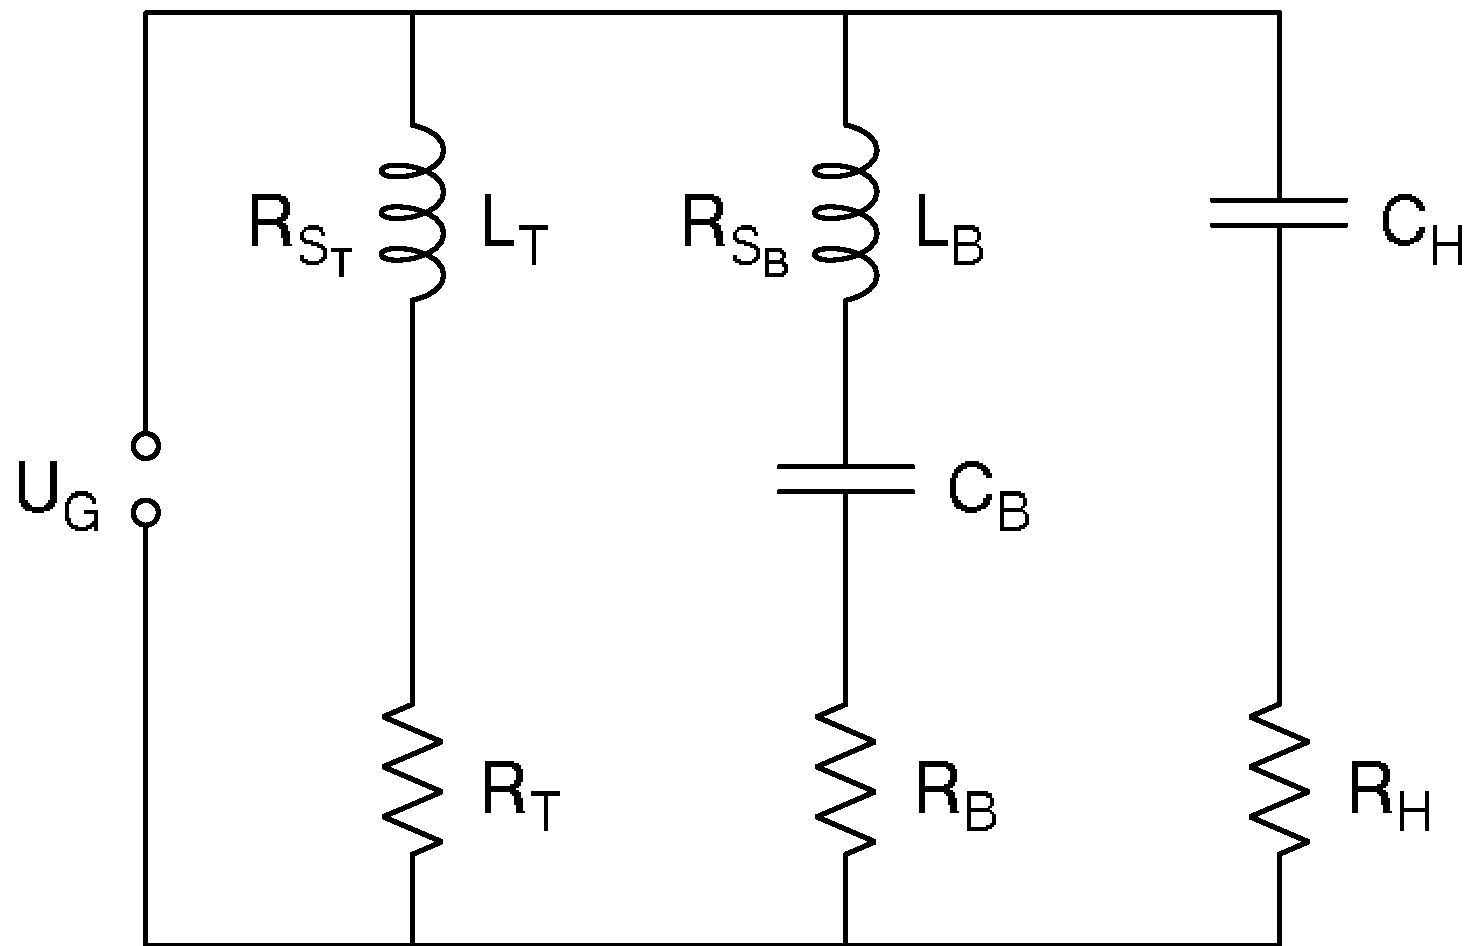
\includegraphics[width=10cm]{frequenzweiche}}
\captionof{figure}{Schaltplan der Frequnzweiche}%
\label{frequenzweiche_schaltplan}
\end{minipage}
\end{center}
Die Einzelnen Komponenten wurden auf ein Steckbrett aufgesteckt und mit Steckbrücken und Bananensteckern verbunden.
\begin{center}
\begin{minipage}{\linewidth}
\centering
\makebox[0cm]{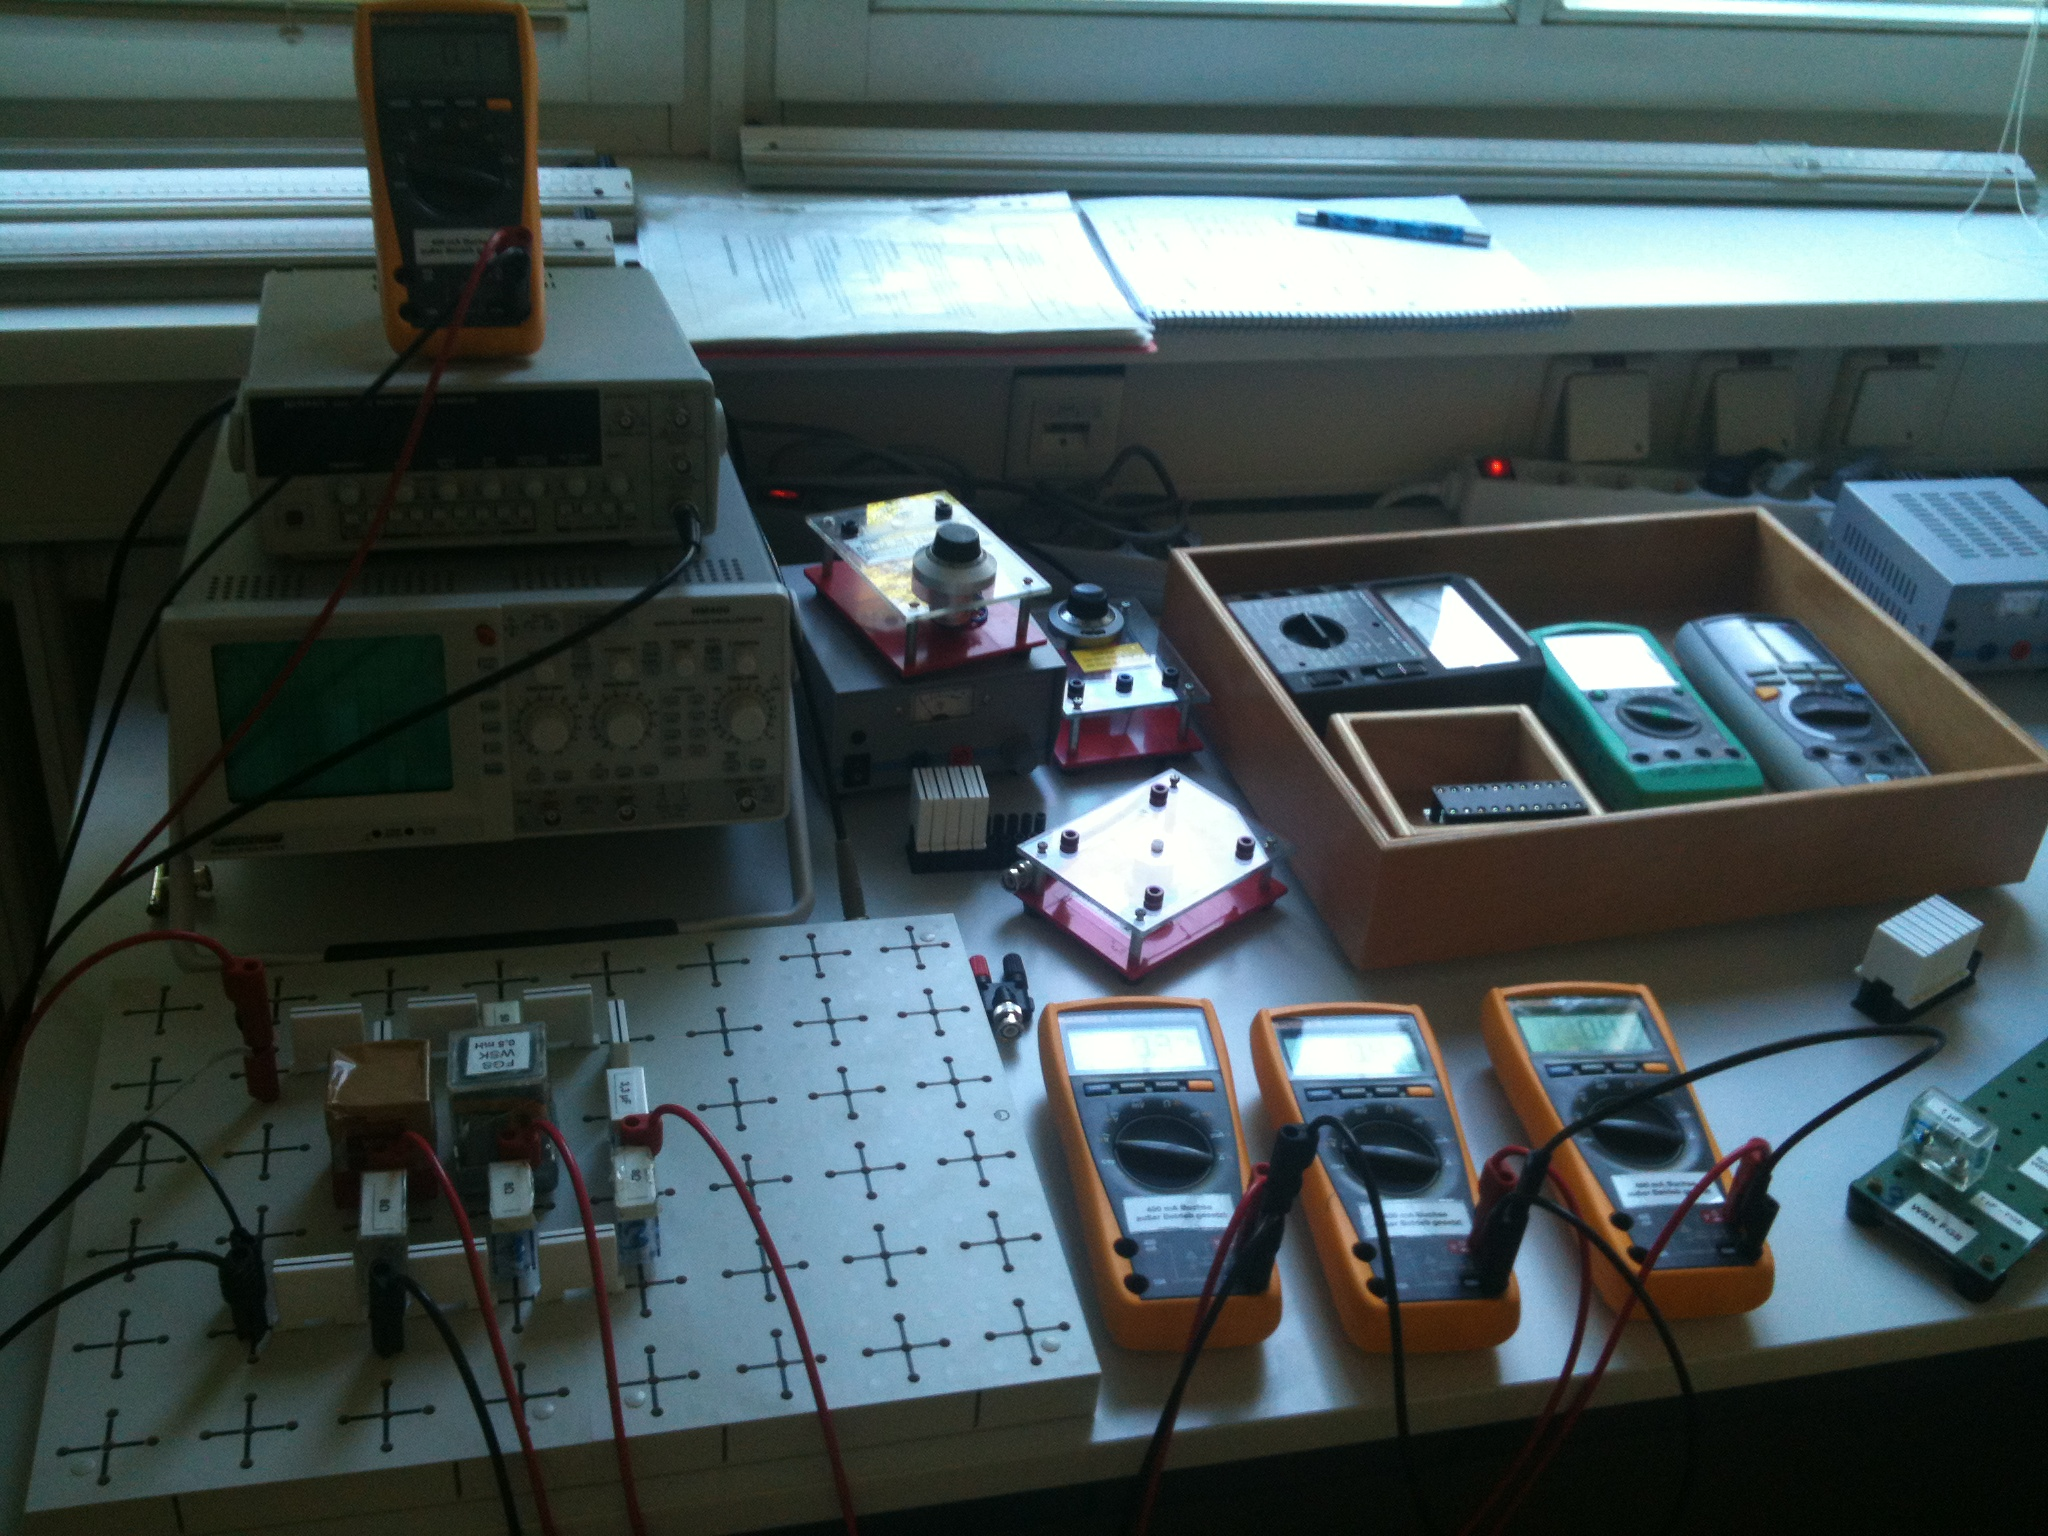
\includegraphics[width=\textwidth]{Bilder/IMG_0027}}
\captionof{figure}{Der Versuchsaufbau}%
\label{frequenzweiche_aufbau}
\end{minipage}
\end{center}
\subsection{Gegebenes}
Um im Anschluss die Messwerte einordnen zu können, wurden folgende Daten separat gemessen:
\begin{center}
\begin{tabular}{c|c}
Messgröße & Messwert\\\hline
\(R_{S_T}\) & \(\left(3,7 \pm 0,5 \right)\, \Omega \) \\
\(L_T\) & \((4,823\pm 0,063)\, mH \) \\
\(R_T\) & \((8,46\pm 0,11)\, \Omega \) \\
\(R_{S_B}\) & \(\left(1,0 \pm 0,5 \right)\, \Omega \) \\
\(L_B\) & \((487\pm 10)\, \mu H \) \\
\(C_B\) & \((38,08\pm 0,32)\, \mu F \) \\
\(R_B\) & \((8,10\pm 0,11)\, \Omega \) \\
\(C_H\) & \((3,172\pm 0,027)\, \mu F \) \\
\(R_H\) & \((8,06\pm 0,11)\, \Omega \) \\
\end{tabular}
\captionof{table}{Sepperate Messung}%
\end{center}
Die Widerstände der Spulen wurden dabei mit dem Voltcraft VC230 gemessen, Kapazitäten, Induktivitäten und die Widerstände der Lastwiderstände hingegen mit dem ELC-131D.
\subsection{Messwerte}
\begin{center}
\begin{tabular}{c|c|c|c|c}
\(f [Hz]\) & \(U_{G} [V]\) & \(U_{R_T} [V]\) & \(U_{R_B} [mV]\) & \(U_{R_H} [mV]\) \\\hline 
\(20.00\) & \(1.513\) & \(1.012\) & \(66.6\) & \(5\) \\ 
\(25.4\) & \(1.513\) & \(1.012\) & \(83.8\) & \(6.3\) \\ 
\(31.9\) & \(1.515\) & \(1.012\) & \(104.3\) & \(7.9\) \\ 
\(39.7\) & \(1.511\) & \(1.008\) & \(128.4\) & \(9.8\) \\ 
\(50.1\) & \(1.509\) & \(1.004\) & \(160.2\) & \(12.3\) \\ 
\(63.8\) & \(1.501\) & \(0.994\) & \(200.7\) & \(15.6\) \\ 
\(79.1\) & \(1.493\) & \(0.984\) & \(244.8\) & \(19.2\) \\ 
\(100.3\) & \(1.481\) & \(0.965\) & \(302.6\) & \(24.2\) \\ 
\(125.2\) & \(1.464\) & \(0.94\) & \(366.5\) & \(29.8\) \\ 
\(159.4\) & \(1.442\) & \(0.902\) & \(447.5\) & \(37.3\) \\ 
\(200.2\) & \(1.41\) & \(0.852\) & \(531.9\) & \(45.8\) \\ 
\(260.3\) & \(1.364\) & \(0.774\) & \(0.636\) & \(57.4\) \\ 
\(319.8\) & \(1.314\) & \(0.697\) & \(0.713\) & \(67.9\) \\ 
\(397.6\) & \(1.253\) & \(0.606\) & \(0.782\) & \(80.5\) \\ 
\(502.2\) & \(1.183\) & \(0.504\) & \(0.84\) & \(95.7\) \\ 
\(635.9\) & \(1.119\) & \(0.409\) & \(0.878\) & \(114.3\) \\ 
\(793.5\) & \(1.074\) & \(0.333\) & \(0.899\) & \(136.2\) \\ 
\(1007\) & \(1.047\) & \(0.267\) & \(0.912\) & \(167.4\) \\ 
\(1254.6\) & \(1.048\) & \(0.22\) & \(0.917\) & \(206.4\) \\ 
\(1589.6\) & \(1.072\) & \(0.182\) & \(0.917\) & \(264.5\) \\ 
\(1999.2\) & \(1.125\) & \(0.154\) & \(0.908\) & \(342.5\) \\ 
\(2574.8\) & \(1.207\) & \(0.13\) & \(0.879\) & \(458.4\) \\ 
\(3135\) & \(1.266\) & \(0.113\) & \(0.828\) & \(565.2\) \\ 
\(3949.5\) & \(1.285\) & \(0.041\) & \(0.721\) & \(682\) \\ 
\(5049.5\) & \(1.197\) & \(0.066\) & \(0.554\) & \(747\) \\ 
\(6394\) & \(1.035\) & \(0.045\) & \(0.4\) & \(731\) \\ 
\(8026.7\) & \(0.854\) & \(0.03\) & \(0.27\) & \(664\) \\ 
\(10016\) & \(0.689\) & \(0.018\) & \(0.179\) & \(575\) \\ 
\(12362\) & \(0.553\) & \(0.011\) & \(0.119\) & \(499\) \\ 
\(15974\) & \(0.432\) & \(0.004\) & \(0.071\) & \(401.7\) \\ 
\(20062\) & \(0.34\) & \(0.001\) & \(0.044\) & \(325.4\)
\end{tabular}


\end{center}
\captionof{table}{Rohmesswerte}
\subsection{Fehlerrechnung}
Die Spannungen wurden mit einem Fluke ??? gemessen, deren Fehler mit \(\Delta U = 1\% +3d\) angegeben war. Daher folgt:
\begin{align}
\Delta \bigg\vert \frac{U_R}{U_G} \bigg\vert &= \sqrt{
\left( \frac{\partial \frac{U_R}{U_G}}{\partial U_G} \right)^2 +
\left( \frac{\partial \frac{U_R}{U_G}}{\partial U_R} \right)^2
}\notag\\
&= \bigg\vert \frac{U_R}{U_G} \bigg\vert \cdot \sqrt{
\left( \frac{\Delta U_G}{U_G} \right)^2 +
\left( \frac{\Delta U_R}{U_R}\right)^2
}
\end{align}
Für den Fehler der Kreisfrequenz \(\omega\) wird die Herstellerangabe \(\Delta f = 0,7 \% \) Herangezogen.
\begin{align}
\omega &= 2 \pi \cdot f\notag\\
\Rightarrow \Delta \omega &= 2 \pi \cdot \Delta f
\end{align}
\subsection{Auswertung}
Um einen Theoretischen Verlauf für die Messung zu erhalten werden nach der {\sc Kirchhoffschen Regel} die Teilspannungen \(U_i\) der Bauelemente mit der Generatorspannung \(U_G\) gleichgesetzt. Für den Hoch-, Band-, und Tiefpass bedeutet das:
\subsubsection{Tiefpass}
\begin{align}
U_G &= U_{R_T} + U_L\notag\\
&= I \cdot Z_R + I \cdot Z_L + I \cdot Z_{R_S}\notag\\
&= I \cdot R_T + I \cdot  R_{S_T} + I \cdot i \omega L\notag\\
\Rightarrow I &= \frac{U_G}{R_T + R_{S_T} + i \omega L}\notag\\
U_{R_T} &= R_T \cdot I\notag\\
&= \frac{R_T \cdot U_G}{R_T + R_{S_T} + i \omega L}\notag\\
\frac{U_{R_T}}{U_G} &= \frac{R_T}{R_T + R_{S_T} + i \omega L}\notag\\
\Rightarrow \bigg\vert \frac{U_{R_T}}{U_G} \bigg\vert &= \frac{R_T}{\sqrt{
\left(\omega L\right)^2 +
\left(R_T + R_{S_T}\right)^2
}} \label{tiefpass}
\end{align}
\subsubsection{Bandpass}
\begin{align}
U_G &= U_{R_B} + U_L + U_C\notag\\
&= I \cdot Z_R + I \cdot Z_L + I \cdot Z_{R_S} + I \cdot Z_C\notag\\
&= I \cdot R_B + I \cdot  R_{S_B} + I \cdot i \omega L_B - I \cdot \frac{i}{\omega C_B} \notag\\
\Rightarrow I &= \frac{U_G}{R_B + R_{S_B} + i \omega L_B - \frac{i}{\omega C_B}}\notag\\
U_{R_B} &= R_B \cdot I\notag\\
&= \frac{R_B \cdot U_G}{R_B + R_{S_B} + i \omega L_B - \frac{i}{\omega C_B}}\notag\\
\frac{U_{R_B}}{U_G} &= \frac{R_B}{R_B + R_{S_B} + i \left( \omega L_B - \frac{1}{\omega C_B}\right)}\notag\\
\Rightarrow \bigg\vert \frac{U_{R_B}}{U_G} \bigg\vert &= \frac{R_B}{\sqrt{
\left(\omega L_B - \frac{1}{\omega C_B} \right)^2 +
\left(R_B + R_{S_B}\right)^2
}} \label{bandpass}
\end{align}
\subsubsection{Hochpass}
\begin{align}
U_G &= U_{R_H} + U_C\notag\\
&= I \cdot Z_R + I \cdot Z_C\notag\\
&= I \cdot R_H - I \cdot \frac{i}{\omega C_H} \notag\\
\Rightarrow I &= \frac{U_G}{R_H - \frac{i}{\omega C_H}}\notag\\
U_{R_H} &= R_H \cdot I\notag\\
&= \frac{R_H \cdot U_G}{R_T - \frac{i}{\omega C_H}}\notag\\
\frac{U_{R_H}}{U_G} &= \frac{R_H}{R_H - \frac{i}{\omega C_H}}\notag\\
\Rightarrow \bigg\vert \frac{U_{R_H}}{U_G} \bigg\vert &= \frac{R_H}{\sqrt{
\left(\frac{1}{\omega C_H} \right)^2 +
\left(R_H\right)^2
}} \label{hochpass}
\end{align}
\subsection{Graphische Auftragung}
Um nun Die Messwerte mit den Theoretischen Vorhersagen zu vergleichen, werden die Graphen von \( \big\vert \frac{U_{R_i}}{U_G} \big\vert \) doppelt logarithmisch aufgetragen und mit den mit Fehlerbalken versehenden Messwerten ergänzt.
\begin{center}
\begin{minipage}{\linewidth}
\centering
\makebox[0cm]{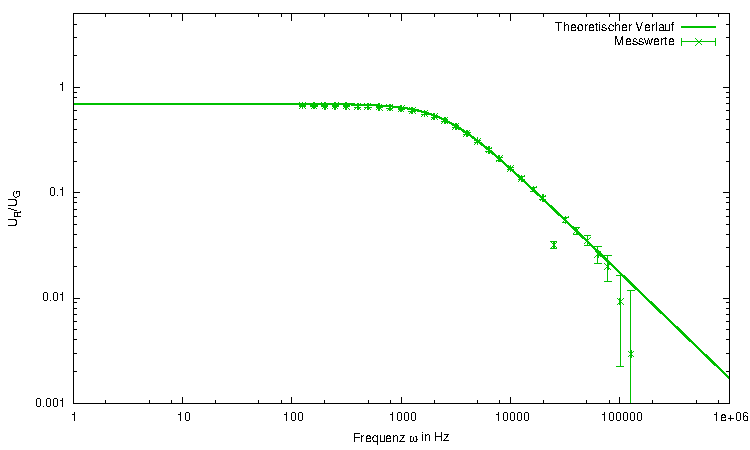
\includegraphics[width=\textwidth]{graphen/tiefpass}}
\captionof{figure}{Messung am Tiefpass}
\end{minipage}
\begin{minipage}{\linewidth}
\centering
\makebox[0cm]{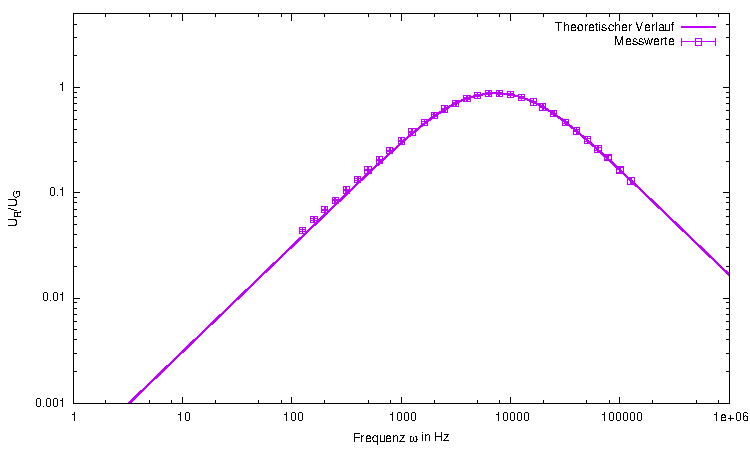
\includegraphics[width=\textwidth]{graphen/bandpass}}
\captionof{figure}{Messung am Bandpass}
\end{minipage}
\begin{minipage}{\linewidth}
\centering
\makebox[0cm]{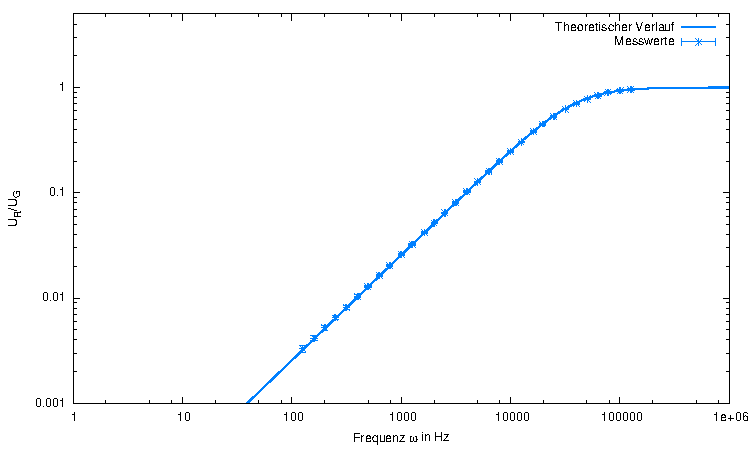
\includegraphics[width=\textwidth]{graphen/hochpass}}
\captionof{figure}{Messung am Hochpass}
\end{minipage}
\end{center}
\subsection{Fazit}
Wie zu sehen ist spiegelt die Theoretische Vorhersage den Echten Verlauf der Frequenzgänge bei Tief-, Band-, und Hochpass sehr gut wieder. Beim Tiefpass ist dabei ein ,,Ausreißer'' zu beobachten. Dieser ist Vermutlich durch ein falsches notieren des Messwerts in der Grafik entstanden. Insgesamt liegt der Graph fast immer im Fehlerintervall der Messpunkte. Die Theoretische Betrachtung kann daher bestätigt werden.